%% Lee
%% In dissertation, change section* to chapter and subsection* to section

\chapter{State-of-the-art}
%\section{State of the art}
\label{sec:State of the art}

For the most part, large scale \acp{ann} have been implemented using \acp{gpu}.
In some cases, such as \acp{cnn}, these \acp{gpu} are quite effective when the \ac{ann} parameters can be reused in the \acp{gpu} local \ac{sram}.

Much of the \ac{asic} and \ac{asip} research has focused on \acp{cnn} \cite{azarkhish2017neurostream}\cite{chen201614}\cite{farabet2011neuflow}. 
In some cases, implementations have focused on solving specific processing ``hot-spots'' \cite{chen201614}.
%% Dissertation
%% convnets use shared parameters that 
%% a) help with translation invariance
%% b) reduce parameter space
%% \acp{cnn} are not always used in face recognition \cite{Taigman_2014_CVPR}
Almost all \ac{asic} and \ac{asip} solutions employ arrays of \acp{pe} each with local processing capability and local memory.
For most of these, the size of the \ac{ann} supported is limited by the size of the local memory or they are limited to \acp{ann} that have reuse opportunities such as \ac{cnn} or have high batch processing opportunities.
In some cases \iffalse, as seen in \fref{fig:Example state-of-the-art die}\fi the area consumed for local memory can exceed 65\% of the 
processing element die \cite{chen2014diannao}\cite{kim2016neurocube}.

Those that employ external \ac{dram}, such as Neurostream \cite{azarkhish2017neurostream}, \ac{tpu} \cite{jouppi2017datacenter}, NnSP{\cite{esmaeilzadeh2005nnsp} and NeuroCube\cite{kim2016neurocube} still 
load weights and \ac{an} states to local \ac{sram} prior to processing, although \ac{tpu} assumes all required parameters can be stored in its very large local \ac{sram}.
Others, such as DianNao \cite{chen2016diannao} are moving away from external \ac{dram} toward \ac{edram}, thereby acknowledging you need both capacity and \ac{dram} bandwidth. 
But \ac{edram} still has capacity and technology availability issues and in the case of \cite{dadiannao2017} still utilizes more than 47\% of the silicon area.

In the case of NnSP{\cite{esmaeilzadeh2005nnsp}, the paper discusses caching data to bridge the speed gap between external memory and the \ac{pe} 
but does not provide details on how to ensure data locality when reading a \ac{dram} cache line and how to minimize the impact of \ac{dram} protocol.
%% dissertion - mention overlapping kernels etc. ????
%%NnSP recognizes the need to stream from SDRAM but does not address the significant issues associated with
%%data structures in \ac{dram} to facilitate streaming and minimize the access protocol limitations of \ac{dram}.

NnSP {\cite{esmaeilzadeh2005nnsp} employs \ac{sdram} but still transfers parameters to a local cache.
There is very little detail regarding network size and supported types but the use of cache implies reuse and therefore suggests shared parameter \acp{ann} such as \acp{cnn}.

Neuflow\cite{farabet2011neuflow} is limited to \acp{cnn} and the external memory is \ac{qdr} \ac{sram} 
and thus will be limited by the network size.

NeuroCube\cite{kim2016neurocube} uses \ac{3dic} along with \ac{hmc} \ac{3ddram} and data is transferred from the \ac{dram} to a \ac{pe}.
The \ac{pe} provides local \ac{sram} which allows NeuroCube\cite{kim2016neurocube} to provide higher performance for shared weight \acp{ann} or batch processing but the performance of \acp{ann} without reuse opportunities are limited by the \ac{hmc} interface bandwidth.

Eyeriss\cite{chen201614} focuses on \acp{cnn} and specifically on the convolution ``hot-spots.''  
It does not support the pooling operations although a local CPU can support these.
However, it does not support the memory intensive fully-connected classifier layers or non-weight-shared locally-connected layers \cite{le2013building}\cite{Taigman_2014_CVPR}.
Eyeriss cannot be effectively applied to locally-connected \acp{ann} such as Deepface \cite{Taigman_2014_CVPR}.

The DianNao family of \acp{asic} \cite{chen2014diannao} \cite{chen2016diannao} originally used external \ac{dram} to store \ac{ann} parameters but still uses \ac{dma} along with \ac{sram} as an intermediate store.
However, the recent versions of the \ac{asic} acknowledge that local \ac{sram} limits the size of the \ac{ann} the device is able to support and have moved from external \ac{dram} to \ac{edram} \cite{dadiannao2017}.
However, the local \ac{edram} is still limited to \SI[per-mode=symbol]{36}{\mega \byte} and therefore requires multiple instances to support \acp{dnn} similar to the types of \ac{dnn} this work is targeting.
To support these useful \acp{dnn}, they have to instantiate up to 64 devices to accommodate the required \ac{dnn} parameter storage resulting in a power approaching \SI[per-mode=symbol]{1}{\kilo\watt} and an area of \SI[per-mode=symbol]{430}{\mm\squared}.
These multi-instance implementations can be used to support batch processing \cite{dadiannao2017} but not the single input systems this work is targeting.

The Neurostream\cite{azarkhish2017neurostream} \ac{asip} uses \ac{3dic} along with \ac{hmc} \ac{3ddram}. 
The Neurostream\cite{azarkhish2017neurostream} acknowledges that \ac{dram} is required to support useful \acp{dnn} but again data is transferred from the \ac{dram} to local \ac{sram} prior to processing.
The local \ac{sram} allows Neurostream\cite{azarkhish2017neurostream} to provide high performance for shared weight \acp{ann} such as \acp{cnn} but the performance of \acp{ann} without reuse opportunities are limited by the \ac{hmc} interface bandwidth.

The Google \ac{tpu} \cite{jouppi2017datacenter} utilizes a large local \SI[per-mode=symbol]{24}{\mega \byte} \ac{sram} along with a 256x256 systolic array and a \SI[per-mode=symbol]{30}{\giga \byte\per\second} external \ac{dram} interface.
It gains performance by storing parameters within the array and by performing large batch processing but acknowledges that it is bandwidth limited when implementing fully-connected \acp{ann}.
It also states that their experience of implementing \acp{ann} in the Google server farms suggests that these fully connected \acp{ann} represent the bulk of their processing requirements.
The simpler \acp{cnn} only represent 5\% of the servers \ac{ann} processing requirements.
It should also be stated that \cite{jouppi2017datacenter} suggests that GPU solutions cannot reach the required performance targets.


%% Dissertation
\iffalse
Unlike the current state-of-the-art, this work focuses on processing data as it read out of the \ac{dram} thus avoiding requiring excessive \ac{sram}.
in the \acp{pe} thus allowing optimum logic assignment to the processing functions.
\fi

\iffalse
The current state-of-the-art does not:
%\vspace{-3mm}
\begin{outline}
  %\itemsep-1.5mm
  \1 currently propose streaming data directly from \ac{3ddram} through the processing functions to avoid the use of large local memory
  \1 propose data structures to support continuous streaming from \ac{dram}
  \1 propose a 3D-stack supporting more than one processing layer
%%  \item provide specific special streaming functions to support a family of \acp{ann}
\end{outline}
%%%
\fi

%% Dissertation
\iffalse
%\vspace{-5mm}
\begin{figure}
\centering
\begin{subfigure}{.45\textwidth}
  \centering
  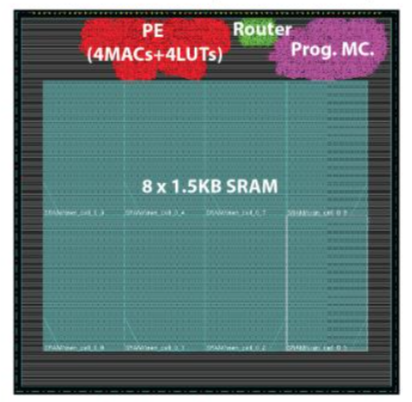
\includegraphics[width=0.8\textwidth]{kim2016neurocube_fig4}
  \captionsetup{justification=centering, skip=6pt}
  \caption{NeuroCube}
  \label{fig:NeuroCubeDie}
\end{subfigure}%
\begin{subfigure}{.45\textwidth}
  \centering
  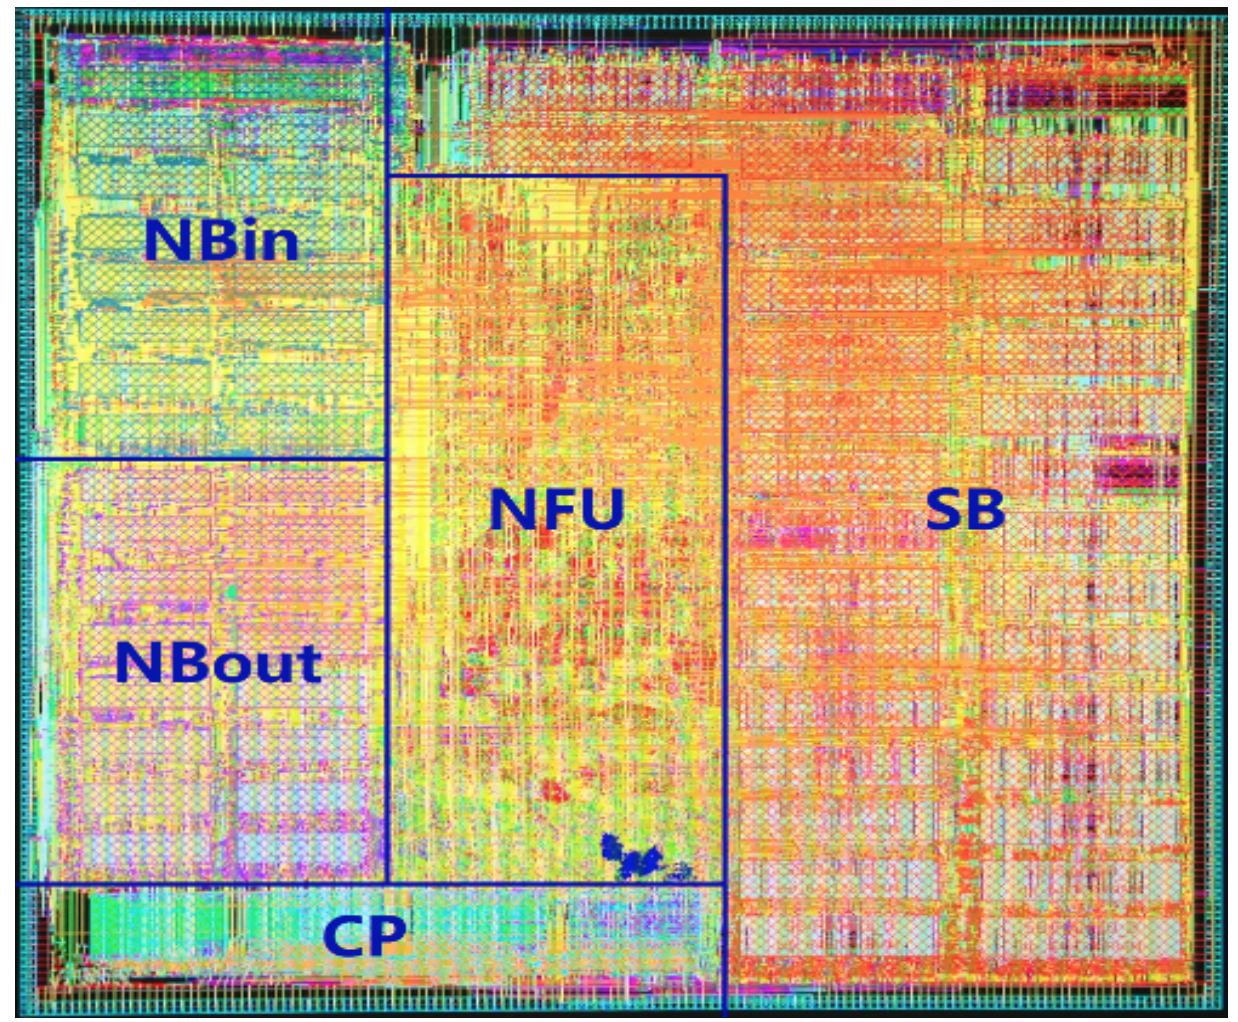
\includegraphics[width=0.8\textwidth]{chen2014diannao_fig15}
  \captionsetup{justification=centering, skip=10pt}
  \caption{Diannao (SB and NBx are \ac{sram})}
  \label{fig:DiannaoDie}
\end{subfigure}
\captionsetup{justification=centering, skip=3pt}
\caption{Example state-of-the-art die}
\label{fig:Example state-of-the-art die}
\end{figure}
%\vspace{-5mm}
\fi


%% Uncomment for dissertation
\iffalse

NeuroCube\cite{kim2016neurocube} is the only solution to explicitly discuss \ac{3d} memory but will be limited by its focus on utilizing local \ac{sram} where our focus is on
providing silicon for processing and not local storage.
Neuflow\cite{farabet2011neuflow} has processing elements that are limited to \acp{cnn}.
NnSP{\cite{esmaeilzadeh2005nnsp} transfers weights and inputs to local \ac{pe} memory prior to processing.
nn-X\cite{gokhale2014240} limits the number format to integer, and although there is some acceptance that similar
results can be obtained compared to floating point, this will likely limit the application space. 
nn-X is also limited to performing the convolution operation and \ac{sram} size will limit its capability when performing the classifier stage.

Below is a summary of current technology.

\section[NnSP]{NnSP{\cite{esmaeilzadeh2005nnsp}}}

Uses external \ac{dram} with a cache.
Does not address the main issue of DRAM access limitations and providing data structures.
It simply says ``use a cache'' but doesn't justify locality issues.

Transfers weights and inputs to local \ac{pe} prior to processing
Similar ``Streaming'' terminology but streams from local memory.
\ac{an} outputs are kept locally and transferred to other \ac{an} via an  \ac{noc}.

No detail on processing element but likely limited to ``standard'' feedforward \acp{ann}.


%% Note: add \section[<section>]{<section> \cite{}} instead of \section{<section> \cite...}
%% to avoid case mismatch issues when running bibtex
\section[NeuroCube]{NeuroCube{\cite{kim2016neurocube}}}
NeuroCube\cite{kim2016neurocube} transfers data to \ac{pe} prior to processing which can limit classifier size although most
convolution kernels can be supported.
The \ac{sram} on the \ac{pe} is significant (see \fref{fig:NeuroCubeDie}).
NeuroCube uses HMC \ac{3ddram} which has limited bandwidth and this will limit network processing performance.
The NeuroCube implements a processing layer but does not address adding additional layers. 

3D uses HMC
 - limited by HMC bandwidth
 - is serdes a good choice for die-to-die communication (typically used for die to chip/board?)
 - doesn't really discuss adding additional layers

Transfers data to \ac{pe} prior to processing


\section[IMAPCAR]{IMAPCAR \cite{kyo2011imapcar}}
IMAPCAR uses external \ac{sram} so will be limited by network size.
The architecture of IMAPCAR is optimized for processing video.

In general will not scale to \acp{ann} of interest.


\section{NeuFlow \cite{farabet2011neuflow}}
Neuflow\cite{farabet2011neuflow} has processing elements that are ``highly optimized'' to \acp{cnn}.
Neuflow is designed around external \ac{qdr} memory and does not address the issues associated with supporting large networks.


\section[nn-X]{nn-X \cite{gokhale2014240}}
nn-X\cite{gokhale2014240} limits the number format to integer, and although there is some acceptance that similar
results can be obtained, this will likely limit the application space. nn-X is also limited to performing the convolution operation
and \ac{sram} size will limit its capability when performing the classifier stage.
nn-X was implemented in an fpga and does not address \ac{sram} size when scaling to larger networks.


\section[Diannao]{Diannao \cite{chen2014diannao}}
Diannao\cite{chen2014diannao} acknowledges the need for large amounts of storage which will exceed the capability of local memory.
The kernel sizes are limited by \ac{sram} size although it does state kernels can be ``broken up.''
The \ac{sram} use on the \ac{pe} is significant (see \fref{fig:DiannaoDie}).


\section[Eyeriss]{Eyeriss \cite{chen201614}}
Eyeris\cite{chen201614} focuses on \acp{cnn} and specifically the convolution stage.
Eyeriss ignores the pooling and classifier stages which although not as compute intensive they are memory intensive.
Therefore Eyeriss limits network size and does not implement the network.

\section[TPU]{TPU \cite{jouppi2017datacenter}}
The TPU utilizes an 256x256 array of \num{64e3} processing elements and demonstrates significant (~30X) performance improvements over \acp{gpu} and \acp{cpu}. It does employ DRAM which provides the required storage capacity
but employs SRAM as an intermediate store between the DRAM and the \acp{pe}.
This Google designed solution acknowledges that it is bandwidth limited when implementing the fully connected \acp{ann}.
It also states that their experience of implementing \acp{ann} in the Google server farms suggests that these fully connected \acp{ann} represent the bulk of their processing requirements.
The simpler \acp{cnn} only represent 5\% of the servers \ac{ann} processing requirements.
It should also be stated that this paper also believes that GPU solutions cannot reach the performance targets even though the GPU community might state otherwise.


\fi



%%%%%%%%%%%%%%%%%%%%%%%%%%%%%%%%%%%%%%%%%%%%%%%%%%%%%%%%%%%%%%%%%%%%%%%%%%%%%%%%%%%%%%%%%%%%%%%%%%%%%%%%%%%%%%%%%%%%%%%
%%%%%%%%%%%%%%%%%%%%%%%%%%%%%%%%%%%%%%%%%%%%%%%%%%%%%%%%%%%%%%%%%%%%%%%%%%%%%%%%%%%%%%%%%%%%%%%%%%%%%%%%%%%%%%%%%%%%%%%
%%%%%%%%%%%%%%%%%%%%%%%%%%%%%%%%%%%%%%%%%%%%%%%%%%%%%%%%%%%%%%%%%%%%%%%%%%%%%%%%%%%%%%%%%%%%%%%%%%%%%%%%%%%%%%%%%%%%%%%
%%%%%%%%%%%%%%%%%%%%%%%%%%%%%%%%%%%%%%%%%%%%%%%%%%%%%%%%%%%%%%%%%%%%%%%%%%%%%%%%%%%%%%%%%%%%%%%%%%%%%%%%%%%%%%%%%%%%%%%
%%%%%%%%%%%%%%%%%%%%%%%%%%%%%%%%%%%%%%%%%%%%%%%%%%%%%%%%%%%%%%%%%%%%%%%%%%%%%%%%%%%%%%%%%%%%%%%%%%%%%%%%%%%%%%%%%%%%%%%
